\documentclass[a4paper,10pt]{article}
\usepackage[american]{babel} % for correct language and hyphenation and stuff
\usepackage[none]{hyphenat}
\usepackage{calc}            % for easier length calculations (infix notation)
\usepackage{enumitem}        % for configuring list environments
\usepackage{fancyhdr}        % for setting header and footer
\usepackage{fontspec}        % for fonts
\usepackage{geometry}        % for setting margins (\newgeometry)
\usepackage{graphicx}        % for pictures
\usepackage{microtype}       % for micro typography stuff
\usepackage{xcolor}          % for colours
\usepackage{lastpage}
\usepackage{fancyhdr}

\usepackage{hyperref}

\fancyhead{}
\fancyfoot{}
\rfoot{\thepage{}~of~\pageref{LastPage}}
\pagestyle{fancy}
\renewcommand{\headrulewidth}{0pt}
\renewcommand{\footrulewidth}{0pt}

% margins
\newgeometry{left=15mm,right=15mm,top=15mm,bottom=15mm}
% width of the gap between left and right column
\newlength{\cvcolumngapwidth}
\setlength{\cvcolumngapwidth}{2mm}
% left column width
\newlength{\cvleftcolumnwidth}
\setlength{\cvleftcolumnwidth}{38mm}
% right column width
\newlength{\cvrightcolumnwidth}
\setlength{\cvrightcolumnwidth}{\textwidth-\cvleftcolumnwidth-\cvcolumngapwidth}
% set paragraph indentation to 0
\setlength{\parindent}{0mm}


% style definitions
% style categories explanation:
% * \cvnameXXX is used for the name;
% * \cvsectionXXX is used for section names (left column, accompanied by a horizontal rule);
% * \cvtitleXXX is used for job/education titles (right column);
% * \cvdurationXXX is used for job/education duration (left column);
% * \cvheadingXXX is used for headings (left column);
% * \cvmainXXX (and \setmainfont) is used for main text;
% * \cvruleXXX is used for the horizontal rules denoting sections.

% font families
\defaultfontfeatures{Ligatures=TeX} % reportedly a good idea, see https://tex.stackexchange.com/a/37251
\newfontfamily{\cvnamefont}{Ubuntu Medium}
\newfontfamily{\cvsectionfont}{Ubuntu Medium}
\newfontfamily{\cvtitlefont}{Ubuntu} % Regular
\newfontfamily{\cvdurationfont}{Ubuntu Light Italic}
\newfontfamily{\cvheadingfont}{Ubuntu} % Regular
\setmainfont{Ubuntu Light}

% colours
\definecolor{cvnamecolor}{rgb}{0.2,0.2,0.2}
\definecolor{cvsectioncolor}{rgb}{0.2,0.2,0.2}
\definecolor{cvtitlecolor}{rgb}{0,0,0}
\definecolor{cvdurationcolor}{rgb}{0,0,0}
\definecolor{cvheadingcolor}{rgb}{0,0,0}
\definecolor{cvmaincolor}{rgb}{0,0,0}
\definecolor{cvrulecolor}{rgb}{0.2,0.2,0.2}
\color{cvmaincolor}

% styles
\newcommand{\cvnamestyle}[1]{{\Large\cvnamefont\textcolor{cvnamecolor}{#1}}}
\newcommand{\cvsectionstyle}[1]{{\normalsize\cvsectionfont\textcolor{cvsectioncolor}{#1}}}
\newcommand{\cvtitlestyle}[1]{{\normalsize\cvtitlefont\textcolor{cvtitlecolor}{#1}}}
\newcommand{\cvdurationstyle}[1]{{\normalsize\cvdurationfont\textcolor{cvdurationcolor}{#1}}}
\newcommand{\cvheadingstyle}[1]{{\normalsize\cvheadingfont\textcolor{cvheadingcolor}{#1}}}

% inter-item spacing
% vertical space after personal info and standard CV items
\newlength{\cvafteritemskipamount}
\setlength{\cvafteritemskipamount}{5mm plus 1.25mm minus 1.25mm}
% vertical space after sections
\newlength{\cvaftersectionskipamount}
\setlength{\cvaftersectionskipamount}{2mm plus 0.5mm minus 0.5mm}
% extra vertical space to be used when a section starts with an item with a heading (e.g. in the skills section), so that the heading does not follow the section name too closely
\newlength{\cvbetweensectionandheadingextraskipamount}
\setlength{\cvbetweensectionandheadingextraskipamount}{1mm plus 0.25mm minus 0.25mm}

% intra-item spacing
% vertical space after name
\newlength{\cvafternameskipamount}
\setlength{\cvafternameskipamount}{3mm plus 0.75mm minus 0.75mm}
% vertical space after personal info lines
\newlength{\cvafterpersonalinfolineskipamount}
\setlength{\cvafterpersonalinfolineskipamount}{2mm plus 0.5mm minus 0.5mm}
% vertical space after titles
\newlength{\cvaftertitleskipamount}
\setlength{\cvaftertitleskipamount}{1mm plus 0.25mm minus 0.25mm}
% value to be used as parskip in right column of CV items and itemsep in lists (same for both, for consistency)
\newlength{\cvparskip}
\setlength{\cvparskip}{0.5mm plus 0.125mm minus 0.125mm}
% set global list configuration (use parskip as itemsep, and no separation otherwise)
\setlist{parsep=0mm,topsep=0mm,partopsep=0mm,itemsep=\cvparskip}

% CV commands
% creates a "personal info" CV item with the given left and right column contents, with appropriate vertical space after
% @param #1 left column content (should be the CV photo)
% @param #2 right column content (should be the name and personal info)

\newcommand{\cvpersonalinfo}[2]{
    % left and right column
    \begin{minipage}[t]{\cvleftcolumnwidth}
        \vspace{0mm} % XXX hack to align to top, see https://tex.stackexchange.com/a/11632
        \raggedleft #1
    \end{minipage}% XXX necessary comment to avoid unwanted space
    \hspace{\cvcolumngapwidth}% XXX necessary comment to avoid unwanted space
    \begin{minipage}[t]{\cvrightcolumnwidth}
        \vspace{0mm} % XXX hack to align to top, see https://tex.stackexchange.com/a/11632
        #2
    \end{minipage}
    % space after
    \vspace{\cvafteritemskipamount}}

% typesets a name, with appropriate vertical space after
% @param #1 name text
\newcommand{\cvname}[1]{
    % name
    \cvnamestyle{#1}
    % space after
    \vspace{\cvafternameskipamount}}

% typesets a line of personal info beginning with an icon, with appropriate vertical space after
% @param #1 parameters for the \includegraphics command used to include the icon
% @param #2 icon filename
% @param #3 line text
\newcommand{\cvpersonalinfolinewithicon}[3]{
    % icon, vertically aligned with text (see https://tex.stackexchange.com/a/129463)
    \raisebox{.5\fontcharht\font`E-.5\height}{\includegraphics[#1]{#2}}
    % text
    #3
    % space after
    \vspace{\cvafterpersonalinfolineskipamount}}

% creates a "section" CV item with the given left column content, a horizontal rule in the right column, and with appropriate vertical space after
% @param #1 left column content (should be the section name)
\newcommand{\cvsection}[1]{
    % left and right column
    \begin{minipage}[t]{\cvleftcolumnwidth}
        \raggedleft\cvsectionstyle{#1}
    \end{minipage}% XXX necessary comment to avoid unwanted space
    \hspace{\cvcolumngapwidth}% XXX necessary comment to avoid unwanted space
    \begin{minipage}[t]{\cvrightcolumnwidth}
        \textcolor{cvrulecolor}{\rule{\cvrightcolumnwidth}{0.5mm}}
    \end{minipage}
    % space after
    \vspace{\cvaftersectionskipamount}}

% creates a standard, multi-purpose CV item with the given left and right column contents, parskip set to cvparskip in the right column, and with appropriate vertical space after
% @param #1 left column content
% @param #2 right column content
\newcommand{\cvitem}[2]{
    % left and right column
    \begin{minipage}[t]{\cvleftcolumnwidth}
        \raggedleft #1
    \end{minipage}% XXX necessary comment to avoid unwanted space
    \hspace{\cvcolumngapwidth}% XXX necessary comment to avoid unwanted space
    \begin{minipage}[t]{\cvrightcolumnwidth}
        \setlength{\parskip}{\cvparskip} #2
    \end{minipage}
    % space after
    \vspace{\cvafteritemskipamount}}

% typesets a title, with appropriate vertical space after
% @param #1 title text
\newcommand{\cvtitle}[1]{
    % title
    \cvtitlestyle{#1}
    % space after
    \vspace{\cvaftertitleskipamount}
    % XXX need to subtract cvparskip here, because it is automatically inserted after the title "paragraph"
    \vspace{-\cvparskip}}


% header and footer
% set "current page number of total page number"
\thispagestyle{fancy}

% preamble end/document start
\begin{document}

% personal info
%\cvpersonalinfo{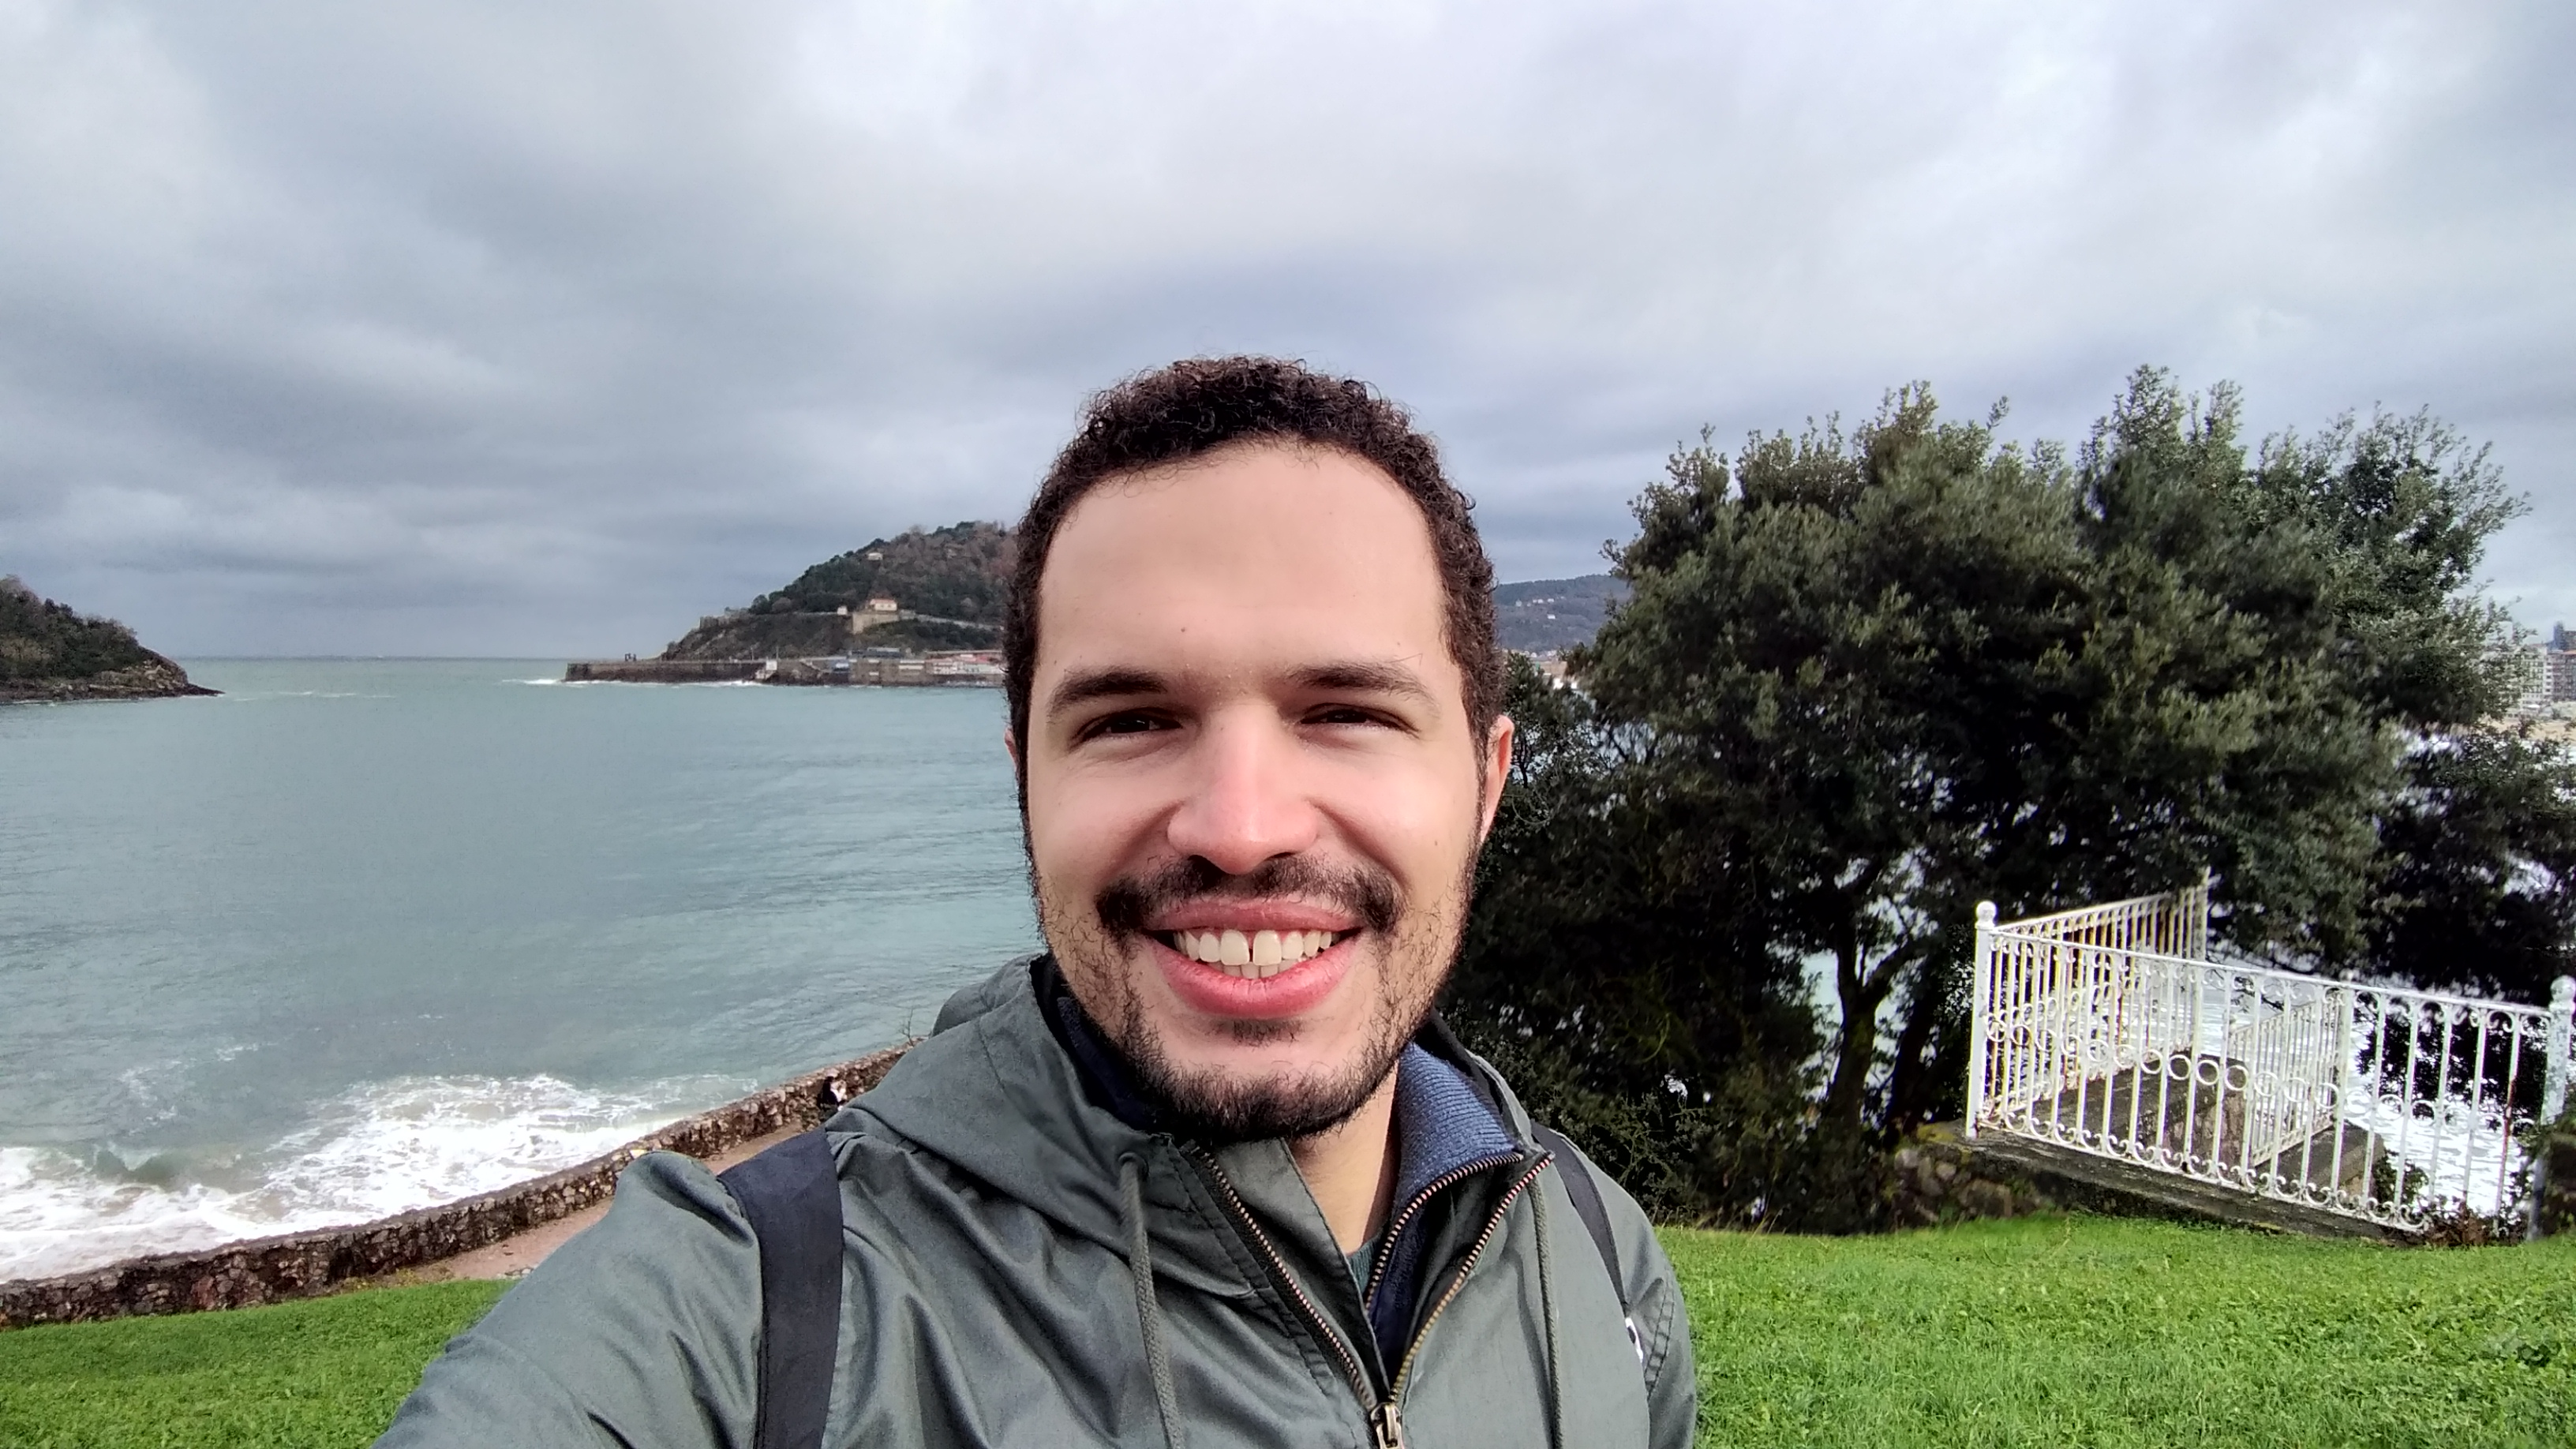
\includegraphics[trim=1000 200 1100 200,clip,scale=0.08]{diego.jpg}} % photo
%\cvpersonalinfo{\includegraphics[angle=-90,trim=600 400 100 400,clip,scale=0.06]{diego2.jpg}} % photo
\cvpersonalinfo{\includegraphics[trim=200 150 50 100,clip,scale=0.06]{02.jpg}} % photo
%\cvpersonalinfo{\includegraphics[trim=450 150 400 500,clip,scale=0.06]{diego4.jpg}} % photo
    {\cvname{Diego Ferreira}
    
    \cvpersonalinfolinewithicon{height=4.5mm}{globe.png}{Belo Horizonte} % address
    
    \cvpersonalinfolinewithicon{height=4.5mm}{phone.png}{+55 31 92000 2151 ou +55 32 98447 0521 (Whatsapp)} % phone number
    
    \cvpersonalinfolinewithicon{height=4.5mm}{envelope.png}{diegobragaferreira@gmail.com} % email address
        
    \cvpersonalinfolinewithicon{height=4.5mm}{github.png}{\href{https://github.com/diegobragaferreira}{/diegobragaferreira}}
    
    \cvpersonalinfolinewithicon{height=4.5mm}{linkedin.png}{\href{https://linkedin.com/in/diego-braga-ferreira}{/in/diego-braga-ferreira}}
    
    \cvpersonalinfolinewithicon{height=4.5mm}{website.png}{\href{https://diegoferreira.net}{diegoferreira.net}}
    
    \cvpersonalinfolinewithicon{height=4.5mm}{scholar.png}{\href{https://scholar.google.com/citations?user=6i7I6wUAAAAJ}{Google Scholar}}
    
    \vspace{0.4cm}
    \cvpersonalinfolinewithicon{height=4.5mm}{comment.png}{
    Sou pesquisador e aluno de Doutorado em Física na Universidade Federal de Minas Gerais, 
    e trabalho em tópicos na área de Informação Quântica, Física da Matéria Condensada e Física Estatística. 
    Minha expertise está relacionada à pesquisa sobre Redes Tensoriais utilizando abordagens analíticas e computacionais, 
    com o objetivo de otimizar sistemas com elevado custo de memória, mesmo para os melhores computadores clássicos, ou utilizando computação na nuvem. 
    Este ferramental teve inspiração em Redes Neurais, bem conhecidos nos últimos anos por serem os responsáveis pela grande evolução nas áreas de 
    Inteligência Artificial e Aprendizado de Máquina.
    \newline\newline
    Nos últimos anos, desenvolvi algoritmos em C++, Matlab, Python e Shell Script, entre outras linguagens, trabalhando com otimização 
    de sistemas complexos, automação de tarefas, e projetos pessoais para a Web.
    \newline\newline
    Tenho versatilidade e criatividade para resolver problemas, além de sólidos conhecimentos sobre linguagens de programação em geral.
    \newline\newline    
    Atualmente estou realizando o programa de cursos da IBM voltado para Engenharia de Dados, oferecido na plataforma Coursera, 
    com objetivo de realizar transição de carreira para algo que tenho verdadeira paixão.
    }}
    
% \cvsection{Area of research}
% 
% \cvitem{\cvdurationstyle{}}
%     {\cvtitle{}
%     Quantum Information, Condensed Matter and Statistical Physics.
%     }    
% 
% \cvsection{Topics of Interest}
% 
% \cvitem{\cvdurationstyle{}}
%     {\cvtitle{}
%     \begin{itemize}[leftmargin=*]
%     \item Many-body localization and thermalisation;
%     \item Open dissipative dynamics;
%     \item Tensor networks renormalization algorithms and numerical methods for time evolution of closed and open systems, for both 1D and 2D;
%     \item Quantum phase transitions;
%     \item Quantum correlations in systems of indistinguishable particles;
%     \item The fermionic extended Hubbard model.
%     \end{itemize}}

% education
\cvsection{Formação Acadêmica}
% phd
\cvitem{\cvdurationstyle{2016 - Presente}}
    {\cvtitle{Doutorado em Física}

    Universidade Federal de Minas Gerais.
    
        \begin{itemize}[leftmargin=*]
        \item \textit{Área:} Informação Quântica.
        \end{itemize}
    }
% master
\cvitem{\cvdurationstyle{2014 - 2016}}
    {\cvtitle{Mestrado em Física}

    Universidade Federal de Minas Gerais.
    
    \begin{itemize}[leftmargin=*]
        \item \textit{Área:} Informação Quântica.
        \end{itemize}
    }
% bachelor
\cvitem{\cvdurationstyle{2010 - 2013}}
    {\cvtitle{Bacharelado em Física com ênfase em Física Computacional}

    Universidade Federal de São João del-Rei.
    
    \begin{itemize}[leftmargin=*]
    \item \textit{Área:} Teoria Quântica de Campos.
    \end{itemize}
    }

\cvsection{Formação Complementar}
% data engineer
\cvitem{\cvdurationstyle{2021 - Em andamento}}
    {\cvtitle{\textit{IBM Data Engineering Professional Certificate}}

    Realizado pelo Coursera.
    
        \begin{itemize}[leftmargin=*]
        \item \textit{Descrição:}   
\includegraphics[clip,scale=0.08]{data-engineering-essentials.png} 
                                    
\includegraphics[clip,scale=0.08]{python-for-data-science-and-ai.png}        
        Estou cursando o programa de cursos integrados de Engenharia de dados da IBM disponibilizado na plataforma Coursera. 
        Este programa traz capacitação essencial para o projeto, implantação e a administração, tanto de dados estruturados quanto de não estruturados. 
        Ele permite desenvolver, na prática, processos como \textit{ETL} utilizando Python e Shell Script, trabalhar com Bancos de Dados Relacionais, 
        consultas em \textit{SQL}, Bancos de Dados \textit{NoSQL}, \textit{Big Data} utilizando Hadoop e Spark, \textit{Data Warehouses},
        ferramentas de \textit{BI}, entre outras coisas.
        \end{itemize}
    }

\newpage
% professional experience
\cvsection{Experiência Profissional}
\cvitem{\cvdurationstyle{2014 - Presente}}
    {\cvtitle{Pesquisador em Informação Quântica --- UFMG (Minas Gerais, Brasil)}
    
    \begin{itemize}[leftmargin=*]
        \vspace{0.2cm}
        
        \item Durante minha trajetória acadêmica, trabalhei em diversos projetos que foram publicados em 7 trabalhos e 3 artigos científicos. 
        Em meu trabalho principal, desenvolvi algoritmos, principalmente em C++, com técnicas de otimização de sistemas de muitas partículas. 
        Este trabalho resultou em uma ferramenta original e eficiente para o estudo completo de um sistema quântico de muitas partículas. 
        Também foram utilizadas a linguagem Shell Script e Matlab, para a geração de um conjunto grande de dados simulados feitos em paralelo 
        e para acessar este conjunto de forma ótima e organizada, possibilitando as análises necessárias. 
        A comunicação e colaborações também foram importantes, tanto interna quanto de pesquisadores internacionais que criaram e desenvolveram a biblioteca utilizada.
        \newline\newline
        Tive a oportunidade de apresentar este trabalho em dois congressos internacionais, sendo, um deles, considerado o mais importante da área, 
        e que foi avaliado e elogiado por outros pesquisadores. 
        Por meio dele tive a oportunidade de conhecer novas técnicas do estado da arte utilizadas em otimização sobre estes problemas.
        \newline\newline
        
        \item \textit{Hard Skills:} 
            \begin{itemize}
            \item Pesquisa científica;
            \item Modelagem;
            \item Otimização;
            \item Automação para gerar e produzir dados.
            \end{itemize}
        \item \textit{Soft Skills:}    
            \begin{itemize}
            \item Comunicação;
            \item Trabalho em equipe e colaboratividade; 
            \item Apresentação de resultados científicos (em português ou inglês); 
            \item Elaboração de textos científicos (em português ou inglês).
            \end{itemize}
    \end{itemize}
    
    }
    
\cvitem{\cvdurationstyle{2020 - Presente}}
    {\cvtitle{Projeto Pessoal de Site e API}
    
    \begin{itemize}[leftmargin=*]
        \vspace{0.2cm}
    
    \item Com o objetivo de organizar investimentos financeiros, desenvolvi uma API que disponibiliza os dados históricos de todas as negociações realizadas no Ibovespa, e no Tesouro Direto.
    Ela é de uso pessoal, e foi feita em C++ utilizando o protocolo \textit{FastCGI} para comunicação com servidor \textit{Nginx} mantido por mim. 
    Os dados são coletados com Shell scripts e armazenados em \textit{flat files} conservando seu formato. Desenvolvi também programas em Javascript/Typescript 
    para calcular e manejar o rendimento de uma carteira. Este projeto pessoal tem como objetivo a criação de um site que possa fazer isso com facilidade, com frontend
    feito em \textit{react} e utilizando \textit{firestore}.
    \newline\newline
    \item \textit{Hard Skills:} 
            \begin{itemize}
            \item Segurança e manutenção de servidor;
            \item Coleta e armazenamento de dados com Shell script;
            \item API em C++ para \textit{queries} personalizadas;
            \item Programação em Javascript/Typescript.
            \end{itemize}
    \end{itemize}
    }
    
% languages
\cvsection{Idiomas}
\cvitem{\cvdurationstyle{}}
    {\cvtitle{}
    
    \begin{itemize}[leftmargin=*]
        \item \textit{Inglês:} Proficiência profissional.
        
        \end{itemize}
    }
% scientific production
% \cvsection{Produção Científica}
% 
% \cvitem{\cvdurationstyle{Preprint}}
%     {\cvtitle{Quantum correlations, entanglement spectrum and coherence of two-particle reduced density matrix in the Extended Hubbard Model}
%     
%     \vspace{0.2cm}
%     \underline{Diego L. B. Ferreira}, Tiago O. Maciel, Reinaldo O. Vianna e Fernando Iemini.
%     
%     \vspace{0.2cm}
%     arXiv:2111.00085 (2021)
%     \textit{submetido à revista Physical Review B}}
% 
% \cvitem{\cvdurationstyle{Journal}}
%     {\cvtitle{Determination of the critical exponents in dissipative phase transitions: coherent anomaly approach}
%     
%     \vspace{0.2cm}
%     Jiasen Jin, Wen-Bin He, Fernando Iemini, \underline{Diego Ferreira}, Ying-Dan Wang, Stefano Chesi e Rosario Fazio.
%     
%     \vspace{0.2cm}
%     Physical Review B, 104 (2021) 214301}
%     
% \cvitem{\cvdurationstyle{Preprint}}
%     {\cvtitle{Quantum Statistical Complexity Measure as a Signalling of Correlation Transitions}
%     
%     \vspace{0.2cm}
%     Andr\'e T. Ces\'ario, \underline{Diego L. B. Ferreira}, Tiago Debarba, Fernando Iemini, Thiago O. Maciel e Reinaldo O. Vianna.
%     
%     \vspace{0.2cm}
%     arXiv:2002.01590 (2020)}
%         
% \cvitem{\cvdurationstyle{Preprint}}
%     {\cvtitle{Probing Genuine Multipartite Entanglement in Large Systems}
%     
%     \vspace{0.2cm}
%     Lucas B. Vieira, \underline{Diego L. Braga Ferreira}, Thiago O. Maciel e Reinaldo O. Vianna.
%     
%     \vspace{0.2cm}
%     arXiv:1911.04649 (2019)}
%         
% \cvitem{\cvdurationstyle{Journal}}
%     {\cvtitle{Completely positive maps for reduced states of indistinguishable particles}
%     
%     \vspace{0.2cm}
%     Leonardo da Silva Souza, Tiago Debarba, \underline{Diego L. Braga Ferreira}, Fernando Iemini e Reinaldo O. Vianna.
%     
%     \vspace{0.2cm}
%     Physical Review A, 98 (2018) 052135}
%     
% % posters
% \cvitem{\cvdurationstyle{Poster}}
%     {\cvtitle{Tensor Network Techniques applied in the Extended
%     Hubbard Model}
%     
%     \vspace{0.2cm}
%     \underline{Diego L. Braga Ferreira}, Thiago O. Maciel, Fernando Iemini e Reinaldo O. Vianna.
%     
%     \vspace{0.2cm}
%     Apresentado no congresso ``Tensor Network based approaches to Quantum Many-Body Systems'', Donostia International Physics Center, Donostia-San Sebasti\'an, Espanha (2019).}
%     
% \cvitem{\cvdurationstyle{Poster}}
%     {\cvtitle{Tensor Network Techniques applied in the Extended
%     Hubbard Model}
%     
%     \vspace{0.2cm}
%     \underline{Diego L. Braga Ferreira}, Thiago O. Maciel, Fernando Iemini e Reinaldo O. Vianna.
%     
%     \vspace{0.2cm}
%     Apresentado na escola ``Summer School on Collective Behaviour in Quantum Matter'', ICTP, Trieste, Itália (2018).}

% references
% \cvsection{References}
% 
% \cvitem{\cvdurationstyle{}}
%     {\cvtitle{Prof. Reinaldo Oliveira Vianna}
%     
%     \emph{Infoquant} Quantum Information Group, Federal University of Minas Gerais (Brazil, Minas Gerais)
%     
%     \vspace{0.2cm}
%     Email: reinaldo@fisica.ufmg.br}
% 
% \cvitem{\cvdurationstyle{}}
%     {\cvtitle{Prof. Fernando Iemini}
%     
%     Physics Institute, Fluminense Federal University (Brazil, Niter\'oi)
%     
%     \vspace{0.2cm}
%     Email: fiemini@mail.if.uff.br}
% 
% \cvitem{\cvdurationstyle{}}
%     {\cvtitle{Dr. Thiago O. Maciel}
%     
%     GIQSUL, Federal University of Santa Catarina (Brazil, Santa Catarina)
%     
%     \vspace{0.2cm}
%     Email: maciel@gmail.com}
\end{document}
